% Consolidated 01-mechanics-kinematics from 2bcf7e8f8b8ab792312bb68085af56aedb51e18b; original TeX fragments preserved.

% === BEGIN 01-mechanics-kinematics-001-020.tex blob 6ce43a6aa2e32d454e1acd3ca861b31e2b39206d ===
\exproblem{1}{1}
一艘汽艇顺流行驶，在 $A$ 点赶上随水漂流的木筏。经过 $\tau=60\,\mathrm{min}$ 后汽艇掉头，在距 $A$ 点 $\ell=6.0\,\mathrm{km}$ 处再次与木筏相遇。设汽艇相对水的航速大小不变，求河流速度。

\exsolution
设水流速度为 $u$，汽艇相对水速为 $v$。改在随木筏一起漂移的参考系中观察，木筏静止，汽艇先以 $v$ 行驶 $\tau$，再以相同的速率返航，因此返航时间同样为 $\tau$。木筏在地面系中漂移距离 $\ell=u(2\tau)$，即
\[
\boxed{u=\frac{\ell}{2\tau}=\frac{6.0\,\mathrm{km}}{2.0\,\mathrm h}=3.0\,\mathrm{km/h}.}
\]

\excheck
结果与汽艇相对水的速率无关，只要求顺、逆行驶时该速率的大小相同。


\exproblem{2}{1--2}
质点以速率 $v_0$ 走过全程的一半；余下的半程中，前一半\emph{时间}以速率 $v_1$、后一半时间以速率 $v_2$ 运动。求全程平均速率。

\exsolution
记总路程为 $S$。前半程历时 $t_0=S/(2v_0)$。余下半程历时 $t_1$，有
\[
\frac S2=\frac{v_1t_1}2+\frac{v_2t_1}2
\quad\Longrightarrow\quad t_1=\frac{S}{v_1+v_2}.
\]
所以平均速率
\[
\boxed{\bar v=\frac{S}{t_0+t_1}
=\frac{2v_0(v_1+v_2)}{2v_0+v_1+v_2}.}
\]

\excheck
若 $v_0=v_1=v_2$，则 $\bar v=v_0$；不要混淆相等时间与相等路程。


\exproblem{3}{2}
汽车从静止开始以 $a=5.0\,\mathrm{m/s^2}$ 匀加速，随后匀速，最后以同样大小的减速度停车。总时间 $T=25\,\mathrm s$，全程平均速率 $72\,\mathrm{km/h}$。求匀速时间。

\exsolution
加速段和减速段的历时均设为 $t$，最大速度为 $at$，匀速段历时 $T-2t$。由速度—时间图像的面积求得位移
\[
S=\tfrac12at^2+at(T-2t)+\tfrac12at^2=at(T-t).
\]
又平均速率为 $20\,\mathrm{m/s}$，故
\[
5t(25-t)=20\times25,\quad(t-5)(t-20)=0.
\]
由于匀速时间非负，有 $t\le12.5\,\mathrm s$，故取 $t=5\,\mathrm s$，
\[
\boxed{T_{\rm uniform}=25-2t=15\,\mathrm s.}
\]

\excheck
最大速率 $25\,\mathrm{m/s}$，总位移 $500\,\mathrm m$，和题给平均速率相符。


\exproblem{4}{2}
质点沿直线单向运动。原书图1.1给出路程—时间曲线，求：（a）全程平均速率；（b）最大瞬时速率；（c）使瞬时速率等于从出发至该时刻平均速率的时刻 $t_0$。
\begin{center}
\begin{tikzpicture}[x=.34cm,y=1.75cm,>=Latex]
\draw[gray!30,step=1] (0,0) grid (20,2);
\draw[->] (0,0)--(21,0) node[right] {$t/\mathrm s$};
\draw[->] (0,0)--(0,2.2) node[above] {$s/\mathrm m$};
\foreach \t in {0,10,20}{\node[below] at (\t,0) {\small\t};}
\foreach \s in {1,2}{\node[left] at (0,\s) {\small\s};}
\draw[very thick,blue!75!black] plot[smooth] coordinates {(0,0)(4,.06)(8,.20)(10,.47)(12,.90)(14,1.40)(16,1.76)(18,1.98)(20,2)};
\draw[dashed] (0,0)--(16,1.76);
\node[above left] at (16,1.76) {$t_0$};
\end{tikzpicture}
\end{center}
以上为根据原图重绘的近似示意，并非原图的精密数字化。

\exsolution
（a）平均速率是两端点连线斜率：
\[
\boxed{\bar v=\frac{2.0\,\mathrm m}{20\,\mathrm s}
=10\,\mathrm{cm/s}.}
\]
（b）瞬时速率是曲线在相应时刻的切线斜率。图中最陡切线斜率约为 $0.25\,\mathrm{m/s}$，所以
\[\boxed{v_{\max}\approx25\,\mathrm{cm/s}.}\]
（c）条件 $v(t_0)=s(t_0)/t_0$ 表示从原点引向曲线的一条切线。按原书图读得
\[\boxed{t_0\approx16\,\mathrm s.}\]

\excheck
后两项为图像估读值；精确拟合应使用原图，而不是本稿示意曲线。


\exproblem{5}{2}
两粒子分别以恒速度矢量 $\bm v_1,\bm v_2$ 运动，初始位矢为 $\bm r_1,\bm r_2$。这些矢量满足什么关系时二者相撞？

\exsolution
若在 $t\ge0$ 相撞，则
\[
\bm r_1+\bm v_1t=\bm r_2+\bm v_2t,
\quad \bm r_1-\bm r_2=(\bm v_2-\bm v_1)t.
\]
当初始不同点且相对速度非零时，必要且充分条件是 $\bm r_1-\bm r_2$ 与 $\bm v_2-\bm v_1$ 同向共线；此时
\[
\boxed{t_{\rm col}=\frac{(\bm r_1-\bm r_2)\cdot(\bm v_2-\bm v_1)}
{\lVert\bm v_2-\bm v_1\rVert^2}>0.}
\]
求出的 $t$ 还须满足上面的矢量方程，单独检验点积正值不够。

\excheck
若初始已重合则 $t=0$ 已相撞；若初始不同点、两速度相同，则永不相撞。


\exproblem{6}{2}
一艘船沿赤道向东航行，速度 $v_0=30\,\mathrm{km/h}$。来自东南方向的风速为 $v=15\,\mathrm{km/h}$，与赤道夹角 $\varphi=60^\circ$。求相对船的风速大小与风向角。

\exsolution
以东、北为 $x,y$ 正方向。东南风吹向西北，所以风的地面速度与船速分别为
\[
\bm v_w=(-v\cos\varphi,v\sin\varphi),\qquad \bm v_s=(v_0,0).
\]
相对风速 $\bm v'=\bm v_w-\bm v_s$，故
\[
\boxed{v'=\sqrt{v_0^2+v^2+2v_0v\cos\varphi}
\approx39.7\,\mathrm{km/h}},
\]
\[
\boxed{\varphi'=\arctan\frac{v\sin\varphi}{v_0+v\cos\varphi}
\approx19.1^\circ}.
\]
相对船的风吹向西偏北约 $19^\circ$。

\excheck
向东行驶的船使相对风的向西分量增大，所以夹角小于原来的 $60^\circ$。


\exproblem{7}{2}
两人从河岸 $A$ 游向正对岸 $B$。甲沿直线 $AB$ 游至终点；乙相对水垂直河流游泳后沿岸步行回 $B$。水速 $v_0=2.0\,\mathrm{km/h}$，二人相对水速 $v'=2.5\,\mathrm{km/h}$。若同时到达，求乙的步速 $u$。

\exsolution
记河宽为 $d$。甲向上游的速度分量必须抵消河流，于是垂直河岸的有效速度为 $\sqrt{v'^2-v_0^2}$，渡河时间
\[
t_A=\frac d{\sqrt{v'^2-v_0^2}}.
\]
乙渡河历时 $d/v'$，顺流漂移 $v_0d/v'$，步行历时 $v_0d/(v'u)$，所以
\[
t_B=\frac d{v'}+\frac{v_0d}{v'u}.
\]
由 $t_A=t_B$，解得
\[
\boxed{u=\frac{v_0}{v'/\sqrt{v'^2-v_0^2}-1}
=\frac{2}{2.5/1.5-1}=3.0\,\mathrm{km/h}.}
\]

\excheck
甲可直线横渡需要 $v'>v_0$；未知河宽 $d$ 被消去。


\exproblem{8}{2--3}
两船从河中浮标分别沿顺流方向和垂直水流方向驶出，均到达距离浮标 $L$ 处后按原路返回。每船相对水的速率是河流速率的 $\eta=1.2$ 倍。求两船往返时间比 $T_A/T_B$。

\exsolution
记船相对水速为 $v$，河速为 $u$。顺河方向往返所需时间
\[
T_A=\frac{L}{v+u}+\frac{L}{v-u}=\frac{2Lv}{v^2-u^2}.
\]
横河方向需以大小 $u$ 的上游分量抵消水流，故有效横向速度是 $\sqrt{v^2-u^2}$，时间
\[
T_B=\frac{2L}{\sqrt{v^2-u^2}}.
\]
相除得
\[
\boxed{\frac{T_A}{T_B}=\frac{v}{\sqrt{v^2-u^2}}
=\frac{\eta}{\sqrt{\eta^2-1}}\approx1.81.}
\]

\excheck
$\eta>1$ 是横河运动可按岸上直线往返的必要条件。


\exproblem{9}{3}
船相对水速比河流速率小 $n=2.0$ 倍。为了使横渡时的顺流漂移最小，相对水的行驶方向应与水流成何角度 $\theta$？

\exsolution
设河宽 $d$、水速 $u$、船相对水速 $v=u/n$，与顺流方向夹角 $0<\theta<\pi$。渡河时间与顺流漂移为
\[
T=\frac d{v\sin\theta},\qquad
\Delta x=(u+v\cos\theta)T
=d\frac{n+\cos\theta}{\sin\theta}.
\]
求导：
\[
\frac{\mathrm d}{\mathrm d\theta}
\frac{n+\cos\theta}{\sin\theta}
=-\frac{1+n\cos\theta}{\sin^2\theta}.
\]
驻点满足 $\cos\theta=-1/n$，且漂移在两侧端点趋于正无穷，故驻点为最小值：
\[
\boxed{\theta=\arccos(-1/n)=120^\circ.}
\]

\excheck
因船速小于水速，不能完全消除顺流漂移，只能使其最小。


\exproblem{10}{3}
同一点同时将两物体分别竖直向上和与水平成 $\theta=60^\circ$ 抛出，初速大小同为 $v_0=25\,\mathrm{m/s}$。忽略空气阻力，求 $t=1.70\,\mathrm s$ 后的间距。

\exsolution
以水平、竖直为坐标轴，两物体的位置分别为
\[
\bm r_1=(0,v_0t-\tfrac12gt^2),\quad
\bm r_2=(v_0t\cos\theta,v_0t\sin\theta-\tfrac12gt^2).
\]
相对位移
\[
\bm r_2-\bm r_1=v_0t(\cos\theta,\sin\theta-1).
\]
取模，并利用 $\cos^2\theta+(1-\sin\theta)^2=2(1-\sin\theta)$：
\[
\boxed{D=v_0t\sqrt{2(1-\sin\theta)}
\approx22.0\,\mathrm m.}
\]

\excheck
两物体重力加速度相等，相对加速度为零；最后结果不依赖 $g$。


\exproblem{11}{3}
两质点同地同刻出发，以 $v_1=3.0\,\mathrm{m/s}$ 和 $v_2=4.0\,\mathrm{m/s}$ 的水平初速度反向运动，仅受重力。求两速度矢量互相垂直时的间距。

\exsolution
两速度可写作
\[
\bm v_1(t)=(v_1,-gt),\quad \bm v_2(t)=(-v_2,-gt).
\]
点积为零等价于 $-v_1v_2+g^2t^2=0$，所以
\[
t=\frac{\sqrt{v_1v_2}}g.
\]
二者竖直位移相同，间距就是水平距离，故
\[
\boxed{D=(v_1+v_2)t
=\frac{(v_1+v_2)\sqrt{v_1v_2}}g
\approx2.47\,\mathrm m\simeq2.5\,\mathrm m.}
\]

\excheck
点积条件具有明确的正时刻解；结果量纲为长度。


\exproblem{12}{3}
三个点位于边长为 $a$ 的等边三角形各顶点，并以速率 $v$ 同时运动；第一个始终指向第二个，第二个指向第三个，第三个指向第一个。问何时汇合？

\exsolution
系统始终保持三重旋转对称，故三点组成边长为 $a(t)$ 的等边三角形。设从 $A$ 指向 $B$ 的边方向为 $\bm e$，$A$ 的速度沿 $\bm e$，$B$ 指向第三个点的速度与 $\bm e$ 成 $120^\circ$。边长变化率
\[
\dot a=(\bm v_B-\bm v_A)\cdot\bm e
=v\cos120^\circ-v=-\tfrac32v.
\]
积分至 $a(T)=0$，得到
\[
\boxed{T=\frac{2a}{3v}.}
\]

\excheck
即使每个点沿曲线追逐，三角形边长的缩减速率依然恒定。


\exproblem{13}{3}
质点 $A$ 以恒速率 $v$ 运动，速度始终指向质点 $B$；$B$ 沿直线以恒速率 $u<v$ 运动。初始时 $A$ 的速度垂直于 $B$ 的速度，二者相距 $\ell$。求追及时间。

\exsolution
取 $B$ 的运动方向为 $x$ 轴。设追逐连线与该轴夹角为 $\alpha(t)$，两点距离为 $r(t)$。相对运动在连线上的投影给出
\[
\dot r=u\cos\alpha-v.
\]
到追及时刻 $T$，由 $r(0)=\ell$、$r(T)=0$，
\[
\ell=vT-u\int_0^T\cos\alpha\,\mathrm dt.
\]
初始连线与 $B$ 的运动方向垂直，因此两点相遇时 $A$ 的水平位移等于 $B$ 的 $uT$：
\[
v\int_0^T\cos\alpha\,\mathrm dt=uT.
\]
代回前式整理得
\[
\boxed{T=\frac{v\ell}{v^2-u^2}.}
\]

\excheck
$u\to0$ 时退化为 $\ell/v$；$u\to v^-$ 时追及时间趋于无穷。


\exproblem{14}{3}
列车长 $\ell=350\,\mathrm m$，从静止开始以 $a=3.0\times10^{-2}\,\mathrm{m/s^2}$ 匀加速。$t_1=30\,\mathrm s$ 时车头灯点亮（事件1），再过 $\tau=60\,\mathrm s$ 后车尾灯点亮（事件2）。求两事件在列车附着系和地面系中的空间间隔；求使它们在同一坐标位置发生的匀速参考系速度。

\exsolution
以初始车尾为原点、列车前进方向为正，车头与车尾的地面坐标为
\[
x_H(t)=\ell+\tfrac12at^2,\quad x_T(t)=\tfrac12at^2.
\]
列车附着坐标中事件1在车头、事件2在车尾，故空间间距为 $\boxed{350\,\mathrm m}$。
地面系中 $t_2=t_1+\tau=90\,\mathrm s$，
\[
x_1-x_2=\ell+\tfrac12a(t_1^2-t_2^2)
=\ell-a\tau(t_1+\tau/2)
=350-108=\boxed{242\,\mathrm m}.
\]
若新惯性系以速度 $V$ 匀速运动，则 $x'=x-Vt$。令 $x_1'=x_2'$ 得
\[
\boxed{V=\frac{x_2-x_1}{\tau}=-\frac{242}{60}
\approx-4.03\,\mathrm{m/s}.}
\]

\excheck
负号表示与列车前进方向相反；车厢附着系是加速系而非惯性系。


\exproblem{15}{3}
电梯从静止开始以 $a=1.2\,\mathrm{m/s^2}$ 向上匀加速，轿厢高 $h=2.7\,\mathrm m$。$2.0\,\mathrm s$ 后天花板一颗螺栓掉落。求：（a）落至地板的时间；（b）在电梯井参考系内螺栓的位移和路程。

\exsolution
脱落瞬间螺栓具有向上的地面速度 $v_0=at_0=2.4\,\mathrm{m/s}$。相对电梯的加速度向下、大小为 $g+a$，于是
\[
h=\tfrac12(g+a)T^2,\quad
\boxed{T=\sqrt{\frac{2h}{g+a}}\approx0.701\,\mathrm s}.
\]
以竖直向上为正，螺栓地面位移
\[
\Delta y=v_0T-\tfrac12gT^2\approx-0.725\,\mathrm m.
\]
脱落后它先上升，在 $t_*=v_0/g\approx0.245\,\mathrm s$ 时转而下落；最高点相对脱落位置上升
\[
d_\uparrow=\frac{v_0^2}{2g}\approx0.294\,\mathrm m.
\]
因此总路程为上升加下降长度：
\[
\boxed{s=2d_\uparrow+|\Delta y|
=\frac{v_0^2}{g}+|\Delta y|\approx1.31\,\mathrm m.}
\]

\excheck
位移约为 $0.73\,\mathrm m$ 向下，路程约 $1.31\,\mathrm m$；二者不能混淆。


\exproblem{16}{3--4}
两质点分别以速率 $v_1,v_2$ 沿两条互相垂直的直线朝交点 $O$ 运动，起初距离 $O$ 分别为 $\ell_1,\ell_2$。求两质点间距达到最小的时刻与最小值。

\exsolution
取两路径为两坐标轴。二者位置为
\[
\bm r_1=(\ell_1-v_1t,0),\quad \bm r_2=(0,\ell_2-v_2t).
\]
间距平方
\[
D^2=(\ell_1-v_1t)^2+(\ell_2-v_2t)^2
\]
是严格凸的二次函数。令 $\mathrm d(D^2)/\mathrm dt=0$，有
\[
\boxed{t_*=\frac{\ell_1v_1+\ell_2v_2}{v_1^2+v_2^2}.}
\]
代回并整理平方，得到
\[
\boxed{D_{\min}=\frac{|\ell_1v_2-\ell_2v_1|}
{\sqrt{v_1^2+v_2^2}}.}
\]

\excheck
若 $\ell_1/v_1=\ell_2/v_2$，两质点同时到达 $O$，最短距离为零。


\exproblem{17}{4}
由公路上点 $A$ 开车前往野外点 $B$，$D$ 为 $B$ 到公路的垂足，$BD=\ell$。汽车野外速度是公路速度的 $1/\eta$（$\eta>1$）。应在距 $D$ 多远的 $C$ 点离开公路，才能最快到达？
\begin{center}
\begin{tikzpicture}[scale=.85]
\draw[thick] (0,2)--(7.4,2);
\draw[dashed] (4.7,2)--(6.5,.1);
\draw[thick] (6.5,2)--(6.5,.1);
\node[above] at (.6,2) {$A$};\node[above] at (4.7,2) {$C$};
\node[above] at (6.5,2) {$D$};\node[below] at (6.5,.1) {$B$};
\node[right] at (6.5,1) {$\ell$};
\end{tikzpicture}
\end{center}

\exsolution
设公路速度为 $v$，$AD=L$，$CD=d\in[0,L]$。公路段距离 $L-d$，野外段距离 $\sqrt{d^2+\ell^2}$，总时间
\[
T(d)=\frac{L-d}{v}+\frac{\eta\sqrt{d^2+\ell^2}}{v}.
\]
有
\[
T'(d)=\frac1v\left(-1+\frac{\eta d}{\sqrt{d^2+\ell^2}}\right),\quad
T''(d)=\frac{\eta\ell^2}{v(d^2+\ell^2)^{3/2}}>0.
\]
唯一无约束极小点满足 $\eta d=\sqrt{d^2+\ell^2}$，故
\[
\boxed{CD=\frac{\ell}{\sqrt{\eta^2-1}}.}
\]

\excheck
若 $AD$ 小于上述距离，必须尊重 $d\le AD$，最优解改为从 $A$ 直接驶入野外。


\exproblem{18}{4}
一质点沿 $x$ 轴运动，原书图1.3给出的速度折线经过 $(0,0),(1,1),(3,1),(6,-2),(7,0)$。设 $x(0)=0$，绘出加速度 $a_x$、坐标 $x$ 与路程 $s$ 的时间图像。
\begin{center}
\begin{tikzpicture}[x=.9cm,y=.7cm,>=Latex]
\draw[gray!30,step=1] (0,-2) grid (7,1);
\draw[->] (0,0)--(7.6,0) node[right] {$t$};
\draw[->] (0,-2.2)--(0,1.4) node[above] {$v_x$};
\draw[very thick,blue!75!black] (0,0)--(1,1)--(3,1)--(6,-2)--(7,0);
\foreach \t in {1,2,3,4,5,6,7}{\node[above] at (\t,0) {\scriptsize\t};}
\node[left] at (0,1) {$1$};\node[left] at (0,-2) {$-2$};
\end{tikzpicture}
\end{center}

\exsolution
按折线各段的斜率，先将速度写成
\[
v_x(t)=\begin{cases}
t,&0\le t\le1,\\1,&1<t\le3,\\
4-t,&3<t\le6,\\2t-14,&6<t\le7.
\end{cases}
\]
于是加速度图由四段水平线组成，
\[
\boxed{a_x(t)=\begin{cases}
1,&0<t<1,\\0,&1<t<3,\\-1,&3<t<6,\\2,&6<t<7.
\end{cases}}
\]
在折线的连接点通常不存在普通导数。根据 $x(0)=0$，分段积分且保持连续，得
\[
\boxed{x(t)=\begin{cases}
t^2/2,&0\le t\le1,\\t-1/2,&1<t\le3,\\
5/2+(t-3)-(t-3)^2/2,&3<t\le6,\\
1-2(t-6)+(t-6)^2,&6<t\le7.
\end{cases}}
\]
由于路程是 $\int_0^t|v_x|\,\mathrm dt$，在 $t=4$ 后速度变负，须改变积分符号：
\[
\boxed{s(t)=\begin{cases}
t^2/2,&0\le t\le1,\\t-1/2,&1<t\le3,\\
5/2+(t-3)-(t-3)^2/2,&3<t\le4,\\
3+(t-4)^2/2,&4<t\le6,\\
5+2(t-6)-(t-6)^2,&6<t\le7.
\end{cases}}
\]

\excheck
$x(4)=3$ 为最大坐标，$x(7)=0$；而 $s(4)=3,s(6)=5,s(7)=6$，路程始终不减。


\exproblem{19}{4}
质点在 $T=10.0\,\mathrm s$ 内沿半径 $R=160\,\mathrm{cm}$ 的半圆弧运动。求：（a）平均速率；（b）平均速度矢量模；（c）若切向加速度恒定，平均加速度矢量的模。

\exsolution
半圆弧长 $\pi R$，故平均速率
\[
\boxed{\bar v=\frac{\pi R}{T}\approx50.3\,\mathrm{cm/s}.}
\]
首末位置间位移为直径 $2R$，平均速度矢量的模为
\[
\boxed{\lVert\langle\bm v\rangle\rVert=\frac{2R}{T}=32\,\mathrm{cm/s}.}
\]
切向加速度恒定时，初、末速率 $v_i,v_f$ 满足 $(v_i+v_f)/2=\pi R/T$。由于起终点切线方向相反，速度矢量增量的模为 $v_i+v_f$，故
\[
\boxed{\lVert\langle\bm a\rangle\rVert
=\frac{v_i+v_f}{T}
=\frac{2\pi R}{T^2}\approx10.1\,\mathrm{cm/s^2}.}
\]

\excheck
平均加速度由总速度矢量增量计算，不等于加速度大小的时间平均。


\exproblem{20}{4}
位矢为 $\bm r(t)=\bm b\,t(1-\alpha t)$，$\bm b$ 是恒矢量，$\alpha>0$。求：（a）速度和加速度；（b）返回初始位置所需时间及其间总路程。原书把 $\bm b$ 记为 $\bm a$；为避免与加速度混淆而改用此记法。

\exsolution
微分得
\[
\boxed{\bm v(t)=\bm b(1-2\alpha t),\qquad
\bm a(t)=-2\alpha\bm b.}
\]
初始位置是 $\bm r(0)=\bm0$。求 $t>0$ 满足 $\bm r(t)=\bm0$，得
\[
\boxed{T=\frac1\alpha.}
\]
在 $t_*=1/(2\alpha)$ 速度反向，质点先远离原点后沿同一路径折返。到最远点的距离为
\[
\lVert\bm r(t_*)\rVert
=\left\lVert\bm b\frac1{2\alpha}
\left(1-\frac12\right)\right\rVert
=\frac{\lVert\bm b\rVert}{4\alpha}.
\]
故往返的总路程是此值的两倍：
\[
\boxed{s=\frac{\lVert\bm b\rVert}{2\alpha}.}
\]

\excheck
$\bm b$ 量纲为长度/时间，$\alpha$ 量纲为时间的倒数；总位移为零不代表总路程为零。

% === END 01-mechanics-kinematics-001-020.tex ===

% === BEGIN 01-mechanics-kinematics-021-030.tex blob 1cb9760d51ddf39451150726c6d303962468e3e9 ===
% Irodov, Arihant PDF pp. 13--15; original printed pages 4--6.
% Chinese translation and independently derived worked solutions: problems 21--30.
\exproblem{21}{4}
一质点在 $t=0$ 时从原点沿 $x$ 轴正方向出发，其速度随时间变化为
$v_x=v_0(1-t/\tau)$，其中 $v_0=10.0\,\mathrm{cm/s}$，$\tau=5.0\,\mathrm s$。求：
(a) $t=6.0,10,20\,\mathrm s$ 时的坐标；
(b) 质点距原点 $10.0\,\mathrm{cm}$ 的所有非负时刻；
(c) 前 $4.0\,\mathrm s$ 和 $8.0\,\mathrm s$ 的路程，并作 $s(t)$ 的定性图。
\exsolution
直接积分并利用 $x(0)=0$ 得
\[
 x(t)=\int_0^t v_0(1-u/\tau)\,\mathrm du
 =v_0t\Bigl(1-\frac{t}{2\tau}\Bigr).
\]
以 $\mathrm{cm}$ 和 $\mathrm s$ 计，$x(t)=10t-t^2$，故
\[
 \boxed{x(6)=24\,\mathrm{cm},\quad x(10)=0,\quad
 x(20)=-200\,\mathrm{cm}=-2.00\,\mathrm m.}
\]
距原点 $10\,\mathrm{cm}$ 意味着 $|x(t)|=10\,\mathrm{cm}$，而非只取 $x=10$。
\[
 t^2-10t+10=0\quad\text{或}\quad t^2-10t-10=0.
\]
三组非负根为
\[
 \boxed{t=5-\sqrt{15}\simeq1.13\,\mathrm s,\ \
 5+\sqrt{15}\simeq8.87\,\mathrm s,\ \
 5+\sqrt{35}\simeq10.92\,\mathrm s.}
\]
由于 $t=\tau=5\,\mathrm s$ 时速度反号，不能用位移代替全程路程：
\[
 s(t)=\begin{cases}
 v_0t(1-t/(2\tau)),&0\le t\le\tau,\\
 v_0\tau-v_0t(1-t/(2\tau)),&t\ge\tau .
 \end{cases}
\]
代入得 $\boxed{s(4)=24\,\mathrm{cm},\ s(8)=34\,\mathrm{cm}}$。
曲线前段凹向下，在 $t=5\,\mathrm s$ 处斜率为零，此后凹向上、路程继续增加。
\excheck 对照本版书末答案，第21(a)题的末项印为 $-4.0\,\mathrm m$，与给定
$v_0,\tau,t$ 不相容；依题面逐项代入应为 $-2.00\,\mathrm m$，记录为版本勘误。

\exproblem{22}{4--5}
质点沿 $x$ 轴正方向运动，速率满足 $v=\alpha\sqrt{x}$，$\alpha>0$，且
$x(0)=0$。求：(a) 速率及加速度的时间规律；(b) 质点走过最初 $s$ 米期间的平均速率。
\exsolution
对离开原点后 $x>0$ 的运动分离变量：
\[
 \frac{\mathrm dx}{\sqrt{x}}=\alpha\,\mathrm dt,\qquad
 2\sqrt{x}=\alpha t,
\quad x=\frac{\alpha^2t^2}{4}.
\]
因此
\[
 \boxed{v(t)=\frac{\alpha^2t}{2},\qquad a_x(t)=\frac{\alpha^2}{2}.}
\]
走完路程 $s$ 所需时间为 $T=2\sqrt{s}/\alpha$，所以
\[
 \boxed{\bar v=\frac{s}{T}=\frac{\alpha\sqrt{s}}2.}
\]
\excheck 本题应补充“$t=0$ 后立即开始移动”的物理选解。
数学上 $\dot x=\alpha\sqrt{x}$ 在 $x=0$ 不满足局部 Lipschitz 条件，
还允许先静止任意时间 $t_*$，再取
$x(t)=\alpha^2(t-t_*)^2/4$；单独给出 $x(0)=0$ 不保证唯一性。

\exproblem{23}{5}
质点作直线减速运动，减速度的大小为 $a\sqrt v$，$a>0$ 为常数，
初速 $v_0>0$。求停止前走过的总路程以及停止所需的时间。
\exsolution
在 $v>0$ 阶段，
\[
 \frac{\mathrm dv}{\mathrm dt}=-a\sqrt v,\qquad
 2\sqrt v=2\sqrt{v_0}-at.
\]
当 $v=0$ 时
\[
 \boxed{T=\frac{2\sqrt{v_0}}a.}
\]
用 $\mathrm dt=-\mathrm dv/(a\sqrt v)$ 算路程：
\[
 s=\int_0^T v\,\mathrm dt
   =\frac1a\int_0^{v_0}\sqrt v\,\mathrm dv
   =\boxed{\frac{2v_0^{3/2}}{3a}}.
\]
\excheck $[a]=\mathrm{m}^{1/2}\mathrm{s}^{-3/2}$，
则 $[\sqrt{v_0}/a]=\mathrm s$，$[v_0^{3/2}/a]=\mathrm m$。

\exproblem{24}{5}
质点的位矢为 $\bm r(t)=at\,\bm i-bt^2\,\bm j$，
其中 $a,b>0$。求：(a) 轨迹 $y(x)$；(b) 速度、加速度的矢量及大小；
(c) 二者夹角 $\theta(t)$；(d) 前 $t$ 秒的平均速度矢量及大小。
\exsolution
消去 $t=x/a$，有
\[
 \boxed{y=-\frac b{a^2}x^2},
\]
即过原点且开口朝下的抛物线。
对位矢求导：
\[
 \boxed{\bm v=a\bm i-2bt\bm j,\qquad
 \bm a=-2b\bm j},\quad
 |\bm v|=\sqrt{a^2+4b^2t^2},\quad|\bm a|=2b.
\]
当 $t\ge0$ 时，通过点积计算夹角：
\[
 \cos\theta=\frac{\bm v\cdot\bm a}{|\bm v||\bm a|}
 =\frac{2bt}{\sqrt{a^2+4b^2t^2}},\qquad
 \boxed{\tan\theta=\frac a{2bt}\ (t>0)}.
\]
$t=0$ 时 $\theta=\pi/2$。前 $t$ 秒平均速度为
\[
 \boxed{\bar{\bm v}(t)=\frac{\bm r(t)-\bm r(0)}t
 =a\bm i-bt\bm j,\quad
 |\bar{\bm v}|=\sqrt{a^2+b^2t^2}.}
\]
\excheck 轨迹开口、加速度方向和末态平均速度的负 $y$ 分量互相吻合。

\exproblem{25}{5}
质点运动方程为 $x=at,\ y=at(1-\alpha t)$，
$a,\alpha>0$。求：(a) 轨迹方程；(b) 速度与加速度；
(c) 速度和加速度夹角为 $\pi/4$ 的时刻。
\exsolution
用 $t=x/a$ 消去时间，得到
\[
 \boxed{y=x-\frac{\alpha}{a}x^2}.
\]
微分可得
\[
 \boxed{\bm v=a\bm i+a(1-2\alpha t)\bm j,\qquad
 \bm a=-2a\alpha\bm j}.
\]
加速度沿负 $y$ 轴，所以夹角为锐角 $\pi/4$ 需要
$v_y<0$ 且 $|v_y|=v_x=a$，即 $1-2\alpha t=-1$，于是
\[
 \boxed{t_0=\frac1\alpha}.
\]
\excheck $t_0$ 时 $\bm v=(a,-a)$，与 $\bm a=(0,-2a\alpha)$
的夹角确为 $45^\circ$；不能误取 $t=0$，那时夹角为 $135^\circ$。

\exproblem{26}{5}
质点的平面运动方程为 $x=a\sin\omega t$，
$y=a(1-\cos\omega t)$，其中 $a,\omega>0$。
求：(a) 经过时间 $\tau$ 的路程；(b) 速度与加速度的夹角。
\exsolution
因 $x^2+(y-a)^2=a^2$，运动轨迹是半径为 $a$、
圆心在 $(0,a)$ 的圆。微分：
\[
 \bm v=a\omega(\cos\omega t\,\bm i+\sin\omega t\,\bm j),\quad
 \bm a=a\omega^2(-\sin\omega t\,\bm i+\cos\omega t\,\bm j).
\]
速度大小恒为 $a\omega$，且 $\bm v\cdot\bm a=0$，
因此
\[
 \boxed{s=a\omega\tau,\qquad \angle(\bm v,\bm a)=\frac\pi2.}
\]
\excheck 周期 $2\pi/\omega$ 中路程 $2\pi a$，与圆周长一致。

\exproblem{27}{5}
质点在 $xy$ 平面内受沿负 $y$ 方向的恒定加速度，大小为 $w$，
其运动轨迹为 $y=Ax-bx^2$，$A,b>0$。求经过坐标原点时的速度大小。
\exsolution
取原点对应的时刻为 $t=0$，记初速度分量为 $v_{x0},v_{y0}$。
因为 $a_x=0$、$a_y=-w$，
\[
 x=v_{x0}t,\qquad y=v_{y0}t-\frac12wt^2
 =\frac{v_{y0}}{v_{x0}}x-\frac{w}{2v_{x0}^2}x^2.
\]
与题给轨迹逐项比较：
\[
 \frac{v_{y0}}{v_{x0}}=A,\qquad
 \frac{w}{2v_{x0}^2}=b.
\]
于是
\[
 \boxed{v_{x0}=\sqrt{\frac w{2b}},\quad
 v_{y0}=A\sqrt{\frac w{2b}},\quad
 v_0=\sqrt{\frac{w(1+A^2)}{2b}}.}
\]
\excheck $b$ 的量纲为 $\mathrm m^{-1}$，根号内量纲为
$\mathrm m^2/\mathrm s^2$。若取反向通过原点，相应分量可同时变号而速率不变。

\exproblem{28}{5}
一小物体以初速度矢量 $\bm v_0$ 与水平面成角抛出，忽略空气阻力。
以重力加速度矢量 $\bm g$ 表示：
(a) 位移 $\bm r(t)$；(b) 前 $t$ 秒的平均速度，以及回到发射高度时全程的平均速度。
\exsolution
以抛出点为位移原点，匀加速运动给出
\[
 \boxed{\bm r(t)=\bm v_0t+\frac12\bm g\,t^2,\qquad
 \bar{\bm v}(0,t)=\bm v_0+\frac12\bm g\,t.}
\]
若初速度与重力方向夹角大于 $90^\circ$，抛体能重新穿过发射高度。
由竖直分量归零得飞行时间
\[
 T=-\frac{2(\bm v_0\cdot\bm g)}{g^2}>0.
\]
故
\[
 \boxed{\bar{\bm v}_{\rm flight}=
 \bm v_0-\frac{\bm g(\bm v_0\cdot\bm g)}{g^2}},
\]
正好是初速度在垂直于 $\bm g$ 的平面内的投影。
\excheck 此式没有把沿抛物线的总路程与位移混为一谈。

\exproblem{29}{5--6}
由地面以初速 $v_0$、与水平夹角 $\alpha$ 抛出一物体，忽略空气阻力。
求：(a) 飞行时间；(b) 最大高度、水平射程，二者何时相等；
(c) 轨迹方程；(d) 发射点与最高点处的曲率半径。
\exsolution
取 $x$ 水平、$y$ 竖直向上：
\[
 x=v_0\cos\alpha\,t,\qquad
 y=v_0\sin\alpha\,t-\frac12gt^2.
\]
回到 $y=0$ 的非零根给出
\[
 \boxed{T=\frac{2v_0\sin\alpha}{g},\quad
 H=\frac{v_0^2\sin^2\alpha}{2g},\quad
 L=\frac{v_0^2\sin2\alpha}{g}.}
\]
$H=L$ 且 $0<\alpha<\pi/2$ 时有
$\frac12\sin\alpha=2\cos\alpha$，即
\[
 \boxed{\tan\alpha=4,\quad\alpha=\arctan4\simeq75.96^\circ.}
\]
消元得
\[
 \boxed{y=x\tan\alpha-
 \frac{gx^2}{2v_0^2\cos^2\alpha}}.
\]
平面曲线的曲率半径 $R=v^3/|\bm v\times\bm g|$，
因为 $|\bm v\times\bm g|=gv_0\cos\alpha$，
所以发射点速度为 $v_0$、顶点速度为 $v_0\cos\alpha$ 时分别为
\[
 \boxed{R_{\rm launch}=\frac{v_0^2}{g\cos\alpha},\qquad
 R_{\rm top}=\frac{v_0^2\cos^2\alpha}{g}.}
\]
\excheck 当 $\alpha\to0$ 时 $H\to0$ 且 $L\to0$；
$R_{\rm top}$ 有限但最高点与地面重合，属极限情况。

\exproblem{30}{6}
沿用第29题条件，画出法向加速度大小 $a_n$、切向加速度大小 $|a_\tau|$
以及总加速度在速度方向上的有符号投影 $a_v$ 随时间的大致变化。
\exsolution
速度分量 $v_x=v_0\cos\alpha$、$v_y=v_0\sin\alpha-gt$，
速率 $v(t)=\sqrt{v_x^2+v_y^2}$。用 $\bm a=(0,-g)$ 的点积和叉积，
\[
 \boxed{a_v(t)=a_\tau(t)=-\frac{g(v_0\sin\alpha-gt)}{v(t)},\quad
 |a_\tau|=\frac{g|v_0\sin\alpha-gt|}{v(t)},\quad
 a_n(t)=\frac{gv_0\cos\alpha}{v(t)}.}
\]
在 $t=0$ 时 $a_v=-g\sin\alpha,\ a_n=g\cos\alpha$；
在顶点 $t=T/2$ 时 $a_v=0,\ a_n=g$；
落地前 $a_v=g\sin\alpha,\ a_n=g\cos\alpha$。
故 $a_n(t)$ 关于 $T/2$ 对称、先增后减；
$|a_\tau|$ 先减至零再增；
$a_v$ 从负值连续增加、过零后为正。
\excheck 任意时刻 $a_\tau^2+a_n^2=g^2$，图形的纵坐标不应超过 $g$。
% === END 01-mechanics-kinematics-021-030.tex ===

% === BEGIN 01-mechanics-kinematics-031-040.tex blob 6af7f2da9103986fed07e318c82c579a88054ad3 ===
% Irodov, Arihant PDF pp. 15--16; original printed pages 6--7.
% Problems 31--40. Derivations follow source data, not blindly the printed key.

\exproblem{31}{6}
一小球从静止开始竖直落下，落下高度 $h$ 后与倾角为 $\alpha$ 的光滑斜面
发生完全弹性碰撞。求再次碰到该斜面的位置与首次碰撞点沿斜面的距离。
\exsolution
首次撞击前球速 $v=\sqrt{2gh}$，方向竖直向下。
以沿斜面向下为切向、离开斜面为法向，碰撞前切向速度为 $v\sin\alpha$，
法向速度为 $-v\cos\alpha$。光滑弹性碰撞保持切向速度、反转法向速度，
所以碰后切向和法向初速分别为 $v\sin\alpha$、$v\cos\alpha$。
重力在两个方向上的加速度分别为 $g\sin\alpha$ 和 $-g\cos\alpha$。
再次撞面要求法向位移为零：
\[
 0=v\cos\alpha\,T-\frac12g\cos\alpha\,T^2
 \quad\Longrightarrow\quad T=\frac{2v}{g}.
\]
此时沿斜面位移
\[
 \ell=v\sin\alpha\,T+\frac12g\sin\alpha\,T^2
 =\frac{4v^2\sin\alpha}{g}.
\]
故
\[
 \boxed{\ell=8h\sin\alpha.}
\]
\excheck 取 $\alpha=0$ 得 $\ell=0$，符合水平镜面反弹后落回原地的极限。
此题的“落下高度”按竖直下落的高度理解。

\exproblem{32}{6}
火炮与目标位于同一高度，相距 $L=5.10\,\mathrm{km}$。
炮弹初速 $v_0=240\,\mathrm{m/s}$，不计阻力。问发射后多久击中目标？
\exsolution
同高射程满足
\[
 L=\frac{v_0^2\sin2\theta}{g},\quad
 q=\frac{gL}{v_0^2}\simeq0.8686<1.
\]
因此有两个可行仰角
\[
 \theta_1=\tfrac12\arcsin q\simeq30.15^\circ,\quad
 \theta_2=\tfrac12(\pi-\arcsin q)\simeq59.85^\circ .
\]
弹道飞行时间为 $T=L/(v_0\cos\theta)$，代入分别得到
\[
 \boxed{T_1\simeq24.6\,\mathrm s=0.410\,\mathrm{min},\qquad
 T_2\simeq42.3\,\mathrm s=0.705\,\mathrm{min}.}
\]
\excheck 必须验证 $L\le v_0^2/g$ 才有可行同高弹道。
书末给出的约 $0.41$ 与 $0.71\,\mathrm{min}$ 对应低、高两条弹道。

\exproblem{33}{6}
同一火炮在同一方位角内，以共同初速 $v_0=250\,\mathrm{m/s}$
先后发射两枚炮弹。第一枚仰角 $\theta_1=60^\circ$，
第二枚仰角 $\theta_2=45^\circ$。忽略阻力，求使两弹空中相撞的发射间隔。
\exsolution
设碰撞发生时两枚炮弹已飞行 $t_1,t_2$，其中 $t_1>t_2>0$，
发射间隔 $\Delta=t_1-t_2$。水平位置重合意味着
$t_1\cos\theta_1=t_2\cos\theta_2$；竖直位置重合意味着
\[
 v_0(t_1\sin\theta_1-t_2\sin\theta_2)
 =\frac g2(t_1^2-t_2^2).
\]
由前式置 $t_1=k\cos\theta_2,\ t_2=k\cos\theta_1$，
可将竖直位置方程改写成
\[
 v_0k\sin(\theta_1-\theta_2)
 =\frac g2 k^2(\cos^2\theta_2-\cos^2\theta_1).
\]
由于 $\cos^2\theta_2-\cos^2\theta_1
=(\cos\theta_2-\cos\theta_1)(\cos\theta_2+\cos\theta_1)$，
非零碰撞时间对应
\[
 k=\frac{2v_0\sin(\theta_1-\theta_2)}
 {g(\cos\theta_2-\cos\theta_1)(\cos\theta_2+\cos\theta_1)}.
\]
从而两次发射间隔
\[
 \boxed{\Delta=t_1-t_2=
 \frac{2v_0\sin(\theta_1-\theta_2)}
 {g(\cos\theta_1+\cos\theta_2)}\simeq10.9\,\mathrm s.}
\]
\excheck 将以上 $t_1,t_2$ 代回水平和竖直位置式，两式均相等；
且 $t_1>t_2>0$，故确为后发射炮弹追上前弹的碰撞。


\exproblem{34}{6}
一气球自地面起以恒定竖直速度 $v_0>0$ 上升；
受风影响，其水平速度为 $v_x=ay$，其中 $y$ 是升空高度，$a$ 是常数。
求：(a) 水平漂移 $x(y)$；(b) 总加速度、切向加速度和法向加速度的大小随 $y$ 的变化。
\exsolution
竖直速度 $\dot y=v_0$ 恒定，故
\[
 \frac{\mathrm dx}{\mathrm dy}=\frac{\dot x}{\dot y}=\frac{ay}{v_0}
 \quad\Longrightarrow\quad
 \boxed{x(y)=\frac{ay^2}{2v_0}},
\]
其中取 $x(0)=0$。瞬时速度、加速度为
$\bm v=(ay,v_0)$、$\bm a=(av_0,0)$，
从而
\[
 \boxed{|\bm a|=|a|v_0,\quad
 a_\tau=\frac{a^2yv_0}{\sqrt{a^2y^2+v_0^2}},\quad
 a_n=\frac{|a|v_0^2}{\sqrt{a^2y^2+v_0^2}}.}
\]
这里 $a_\tau$ 为上升阶段的非负切向加速度。
\excheck $a_\tau^2+a_n^2=(av_0)^2$；
$y=0$ 时速度竖直、加速度水平，故 $a_\tau=0$。

\exproblem{35}{6}
质点速度为 $\bm v=a\bm i+bx\bm j$，
$\bm i,\bm j$ 为坐标轴单位矢量，$a,b$ 为常数，
初始位置 $x=y=0$。求：(a) 轨迹 $y(x)$；
(b) 曲率半径 $R(x)$。
\exsolution
当 $a\ne0$，
\[
 \dot x=a,\quad\dot y=bx,\quad
 \frac{\mathrm dy}{\mathrm dx}=\frac{bx}{a}
 \quad\Longrightarrow\quad
 \boxed{y(x)=\frac b{2a}x^2}.
\]
对显函数曲线 $y(x)$，曲率半径为
$R=(1+y'^2)^{3/2}/|y''|$，
所以在 $b\ne0$ 时
\[
 \boxed{R(x)=\left|\frac ab\right|
 \left(1+\frac{b^2x^2}{a^2}\right)^{3/2}.}
\]
\excheck 直接计算加速度 $\bm a=(0,ab)$，
再用 $R=|\bm v|^3/|\bm v\times\bm a|$ 得到同式。
若 $b=0$ 则轨迹为直线、$R=\infty$，公式需按极限解释。

\exproblem{36}{6}
质点沿一条已给定的轨迹单向运动。
设一恒定矢量 $\bm a_0=a\,\bm i$（$a>0$），
实际切向加速度是 $\bm a_0$ 在单位切向 $\bm\tau$
上的投影 $a_\tau=\bm a_0\cdot\bm\tau$（原书图1.4）。
若经过 $x=0$ 时速度可视为零，求速率 $v(x)$。
\exsolution
定义弧长 $s$，则 $v=\mathrm ds/\mathrm dt$、
$a_\tau=v\,\mathrm dv/\mathrm ds$，
且 $\bm\tau\cdot\bm i=\mathrm dx/\mathrm ds$。因此
\[
 v\frac{\mathrm dv}{\mathrm ds}
 =a\frac{\mathrm dx}{\mathrm ds}
 \quad\Longrightarrow\quad
 \frac12\mathrm d(v^2)=a\,\mathrm dx .
\]
将 $v(0)=0$ 作为初始条件积分：
\[
 \boxed{v(x)=\sqrt{2ax}}\quad (x\ge0).
\]
\excheck 结果与轨迹具体形状无关，但只适用于质点确能到达的
$x\ge0$ 区域；原书的简答因根号字体可能易误认，需保留根号。

\exproblem{37}{6--7}
质点沿圆周运动，速率 $v=at$，
$a=0.50\,\mathrm{m/s^2}$。求从静止开始走过圆周长度的
$n=0.10$ 倍时的合加速度大小。
\exsolution
切向加速度为 $a_\tau=\dot v=a$；
圆周弧长 $s(t)=\frac12at^2$。
走过 $n$ 圈对应 $s=2\pi Rn$，
故 $t^2=4\pi Rn/a$。
法向加速度
\[
 a_n=\frac{v^2}{R}=\frac{a^2t^2}{R}=4\pi na .
\]
因此
\[
 \boxed{a_{\rm total}=a\sqrt{1+16\pi^2n^2}
 \simeq 0.80\,\mathrm{m/s^2}.}
\]
\excheck $R$ 最终消去；$n\to0$ 时合加速度趋于 $a$。

\exproblem{38}{7}
质点沿半径 $R$ 的圆周减速运动，在任意时刻其切向与法向
加速度大小相同，初速为 $v_0$。求：
(a) $v(t)$ 和 $v(s)$；(b) 合加速度大小作为 $v$ 或已走路程 $s$ 的函数。
\exsolution
由于正沿轨迹减速，$a_\tau=\dot v=-v^2/R$。
分离变量：
\[
 \int_{v_0}^{v(t)}\frac{\mathrm dv}{v^2}=-\frac tR
 \quad\Longrightarrow\quad
 \boxed{v(t)=\frac{v_0}{1+v_0t/R}}.
\]
又 $\dot v=v\,\mathrm dv/\mathrm ds$，所以
$\mathrm dv/\mathrm ds=-v/R$，得
\[
 \boxed{v(s)=v_0e^{-s/R}}.
\]
合加速度为互相垂直的两分量的平方和开方：
\[
 \boxed{a_{\rm total}(v)=\frac{\sqrt2\,v^2}{R},\qquad
 a_{\rm total}(s)=\frac{\sqrt2\,v_0^2}{R}e^{-2s/R}.}
\]
\excheck 切向减速始终为负，$t\to\infty$ 时速率趋零，
但不会在有限时刻突然停止；$s\to\infty$。

\exproblem{39}{7}
质点沿半径为 $R$ 的圆弧运动，速率随已走弧长 $s$ 变化为
$v=a\sqrt s$，$a$ 为正常数。求合加速度与速度方向的夹角 $\theta(s)$。
\exsolution
切向加速度 $a_\tau=v\,\mathrm dv/\mathrm ds
 =(a\sqrt s)(a/(2\sqrt s))=a^2/2$；
法向加速度 $a_n=v^2/R=a^2s/R$。二者互相垂直，
故在 $s>0$ 时
\[
 \boxed{\tan\theta=\frac{a_n}{a_\tau}=\frac{2s}{R},
 \qquad \theta(s)=\arctan\frac{2s}{R}.}
\]
\excheck 当 $s\to0^+$，角度趋零；
当 $s\gg R$ 时，法向分量占主导，角度趋 $\pi/2$。

\exproblem{40}{7}
质点沿半径为 $R$ 的圆弧运动，其相对起点的有符号弧位移为
$\ell(t)=a\sin\omega t$。给定 $R=1.00\,\mathrm m$、
$a=0.80\,\mathrm m$、$\omega=2.00\,\mathrm{rad/s}$。
求：(a) $\ell=0$ 及 $\ell=\pm a$ 时合加速度大小；
(b) 最小合加速度及相应弧位移。
\exsolution
沿圆弧的速度与切向加速度为
$\dot\ell=a\omega\cos\omega t$、
$a_\tau=\ddot\ell=-\omega^2\ell$。
法向加速度大小
$a_n=(\dot\ell)^2/R=\omega^2(a^2-\ell^2)/R$。
因此
\[
 A^2(\ell)=\omega^4\left[
 \ell^2+\frac{(a^2-\ell^2)^2}{R^2}\right].
\]
当 $\ell=0$ 时 $A=\omega^2a^2/R=2.56\,\mathrm{m/s^2}$；
$\ell=\pm a$ 时 $A=\omega^2a=3.20\,\mathrm{m/s^2}$。
置 $z=\ell^2\in[0,a^2]$ 并对 $A^2$ 求导：
\[
 \frac{\mathrm d}{\mathrm dz}
 \left[z+\frac{(a^2-z)^2}{R^2}\right]
 =1-\frac{2(a^2-z)}{R^2}.
\]
本题 $a^2-R^2/2=0.14\,\mathrm{m^2}>0$，
内点极小值发生于
$\ell_m=\pm\sqrt{a^2-R^2/2}$。故
\[
 \boxed{\ell_m\simeq\pm0.374\,\mathrm m,\qquad
 A_{\min}=\omega^2\sqrt{a^2-\frac{R^2}{4}}
 \simeq2.50\,\mathrm{m/s^2}.}
\]
\excheck 计算表明 $2.50<2.56<3.20$。
一般参数下若 $a^2\le R^2/2$，极小点在 $\ell=0$，
不能不核查区间就套内点公式。
% === END 01-mechanics-kinematics-031-040.tex ===

% === BEGIN 01-mechanics-kinematics-041-050.tex blob ae9b66ecdddce91d2aef3e0867c19b978253778c ===
% Irodov, Arihant PDF pp. 16--17; original printed pp. 7--8.
% Problems 41--50. Source inconsistencies are recorded where relevant.

\exproblem{41}{7}
质点在平面内运动，其切向加速度恒为 $a_\tau=a>0$，
法向加速度为 $a_n=bt^4$，$b>0$；初始时刻静止。
求曲率半径 $R$ 与合加速度大小 $A$ 关于已走路程 $s$ 的表达式。
\exsolution
由初速为零及切向加速度恒定，
\[
 v(t)=at,\qquad s(t)=\frac12at^2.
\]
曲率半径满足 $a_n=v^2/R$，故 $t>0$ 时
\[
 R=\frac{a^2t^2}{bt^4}=\frac{a^2}{bt^2}
 =\boxed{\frac{a^3}{2bs}}.
\]
把 $t^2=2s/a$ 代入法向分量，有
$a_n=bt^4=4bs^2/a^2$。
所以
\[
 \boxed{A(s)=\sqrt{a^2+\frac{16b^2s^4}{a^4}}
 =a\sqrt{1+\left(\frac{4bs^2}{a^3}\right)^2}.}
\]
\excheck 当 $s\to0^+$，$R\to\infty$、
$A\to a$；表示初始瞬间近似直线加速，不意味着轨迹全程为直线。

\exproblem{42}{7}
质点沿一条平面曲线以恒定速率 $v$ 运动。求 $x=0$ 时的法向
加速度大小及曲率半径，其中轨迹分别为：
(a) $y=ax^2$；(b) $x^2/a^2+y^2/b^2=1$（椭圆半轴 $a,b>0$）。
\exsolution
定速运动切向加速度为零，合加速度完全沿主法线，
大小 $A=v^2/R$。
对平面图像 $y(x)$，
\[
 \kappa=\frac{|y''|}{(1+y'^2)^{3/2}},\qquad R=\kappa^{-1}.
\]
(a) $y'=2ax,\ y''=2a$，在 $x=0$ 有 $\kappa=2|a|$，因此
\[
 \boxed{R_a=\frac1{2|a|},\qquad A_a=2|a|v^2.}
\]
(b) 椭圆的 $x=0$ 两点为 $(0,\pm b)$。在顶部附近选正根
$y=b\sqrt{1-x^2/a^2}$，则 $y'(0)=0$、
$y''(0)=-b/a^2$，故
\[
 \boxed{R_b=\frac{a^2}{b},\qquad A_b=\frac{bv^2}{a^2}.}
\]
底部对称点有相同大小。
\excheck 若 $a=0$，(a) 变成直线，取 $R=\infty$、
$A=0$。椭圆两点的加速度均指向曲线的内侧。

\exproblem{43}{7}
质点 $A$ 沿半径 $R=50\,\mathrm{cm}$ 的圆运动；
由圆上一固定点 $O$ 指向质点的位矢 $\bm r=\overrightarrow{OA}$
以恒定角速度 $\omega=0.40\,\mathrm{rad/s}$ 转动（见原书图1.5）。
求质点速率及合加速度大小与方向。
\begin{center}
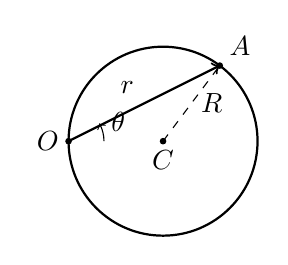
\begin{tikzpicture}[scale=.75]
\coordinate (O) at (0,0);
\coordinate (C) at (1.6,0);
\coordinate (A) at (2.56,1.28);
\draw[thick] (C) circle (1.6);
\draw[->,thick] (O)--(A) node[midway,above left] {$\bm r$};
\draw[dashed] (C)--(A) node[midway,right] {$R$};
\fill (O) circle (1.6pt) node[left] {$O$};
\fill (C) circle (1.6pt) node[below] {$C$};
\fill (A) circle (1.6pt) node[above right] {$A$};
\draw[->] (.6,0) arc (0:30:.6);
\node at (.84,.32) {$\theta$};
\end{tikzpicture}
\end{center}
\exsolution
令 $\theta=\omega t+\theta_0$ 为位矢 $OA$ 与圆心直径 $OC$ 的夹角。
圆心在 $(R,0)$ 时圆的极坐标方程是 $r=2R\cos\theta$。
质点坐标
\[
 x=r\cos\theta=R(1+\cos2\theta),\quad
 y=r\sin\theta=R\sin2\theta.
\]
故质点绕圆心 $C$ 的圆心角速度为 $2\omega$，且恒定。
因此
\[
 \boxed{v=2R\omega=0.40\,\mathrm{m/s}},\qquad
 \boxed{A=\frac{v^2}{R}=4R\omega^2
 =0.32\,\mathrm{m/s^2}}.
\]
\excheck 合加速度始终\emph{沿半径指向圆心 $C$}，并非指向
固定观测点 $O$。图像及解析只在位矢有意义的连续运动段解释。

\exproblem{44}{7}
一轮绕固定轴转动，转角 $\varphi=at^2$，
$a=0.20\,\mathrm{rad/s^2}$。在 $t=2.5\,\mathrm s$ 时，
轮缘点 $A$ 的线速率为 $v=0.65\,\mathrm{m/s}$。
求此刻该点的合加速度大小。
\exsolution
角速度、角加速度分别为
\[
 \omega=2at,\qquad\beta=2a.
\]
轮缘半径由 $v=R\omega$ 得 $R=v/(2at)$。
法向加速度 $a_n=R\omega^2=2at\,v$，
切向加速度 $a_\tau=R\beta=v/t$。
所以
\[
 \boxed{A=\frac vt\sqrt{1+4a^2t^4}
 \simeq0.700\,\mathrm{m/s^2}.}
\]
\excheck 所需半径 $R=0.65\,\mathrm m$，
$a_\tau=0.26\,\mathrm{m/s^2}$、
$a_n=0.65\,\mathrm{m/s^2}$，
勾股合成即 $0.700\,\mathrm{m/s^2}$。

\exproblem{45}{8}
一发炮弹在长 $\ell=2.0\,\mathrm m$ 的炮膛内作匀加速直线运动，
出膛速率 $v=320\,\mathrm{m/s}$。
在炮膛内弹体沿轴向共旋转 $n=2.0$ 圈。求出膛瞬间的自转角速度。
\exsolution
按原书标准求解需采用\emph{等螺距膛线}（弹体每前进相同长度
便转过相同角度）的通常模型。这时累计转角与轴向位移满足
$\varphi=(2\pi n/\ell)x$，故
\[
 \omega_{\rm spin}
 =\frac{\mathrm d\varphi}{\mathrm dt}
 =\frac{2\pi n}{\ell}\frac{\mathrm dx}{\mathrm dt}.
\]
在出膛时
\[
 \boxed{\omega_{\rm spin}=\frac{2\pi n v}{\ell}
 \simeq2.01\times10^3\,\mathrm{rad/s}.}
\]
\excheck 若\emph{只}知道“直线匀加速、共转 $n$ 圈”，
没有等螺距或角加速度规律，实际上不能唯一确定终端角速度。
上述结果以炮膛螺距固定的隐含物理条件为前提。

\exproblem{46}{8}
刚体绕固定轴按 $\varphi=at-bt^2$ 旋转，其中
$a=6.0\,\mathrm{rad/s}$、$b=2.0\,\mathrm{rad/s^2}$。
求：(a) 从 $t=0$ 至第一次停转期间的平均角速度和平均角加速度；
(b) 刚停转时的角加速度。
\exsolution
严格依据\emph{本版所印二次时间规律}，
\[
 \omega=\dot\varphi=a-2bt,\qquad
 \beta=\dot\omega=-2b.
\]
第一次停转时间 $T=a/(2b)=1.5\,\mathrm s$，
累计转角 $\varphi(T)=aT-bT^2=a^2/(4b)$。
因此
\[
 \boxed{\bar\omega=
 \frac{\varphi(T)-\varphi(0)}T=\frac a2
 =3.0\,\mathrm{rad/s},}
\]
\[
 \boxed{\bar\beta=\frac{\omega(T)-\omega(0)}T=-2b
 =-4.0\,\mathrm{rad/s^2},\qquad
 \beta(T)=-4.0\,\mathrm{rad/s^2}.}
\]
\excheck 本版书末给出的 $4\,\mathrm{rad/s}$、
$-6\,\mathrm{rad/s^2}$、$-12\,\mathrm{rad/s^2}$ 等数值
与\emph{印刷题面的二次函数及单位}不符，而与另一个三次时间
模型 $\varphi=at-bt^3$ 的计算相符（此时 $b$ 应为
$\mathrm{rad/s^3}$）。本稿保留原题面并标记此实质性勘误，
不擅自把题面修改为三次方。

\exproblem{47}{8}
刚体从静止起绕固定轴转动，角加速度随时间变化为
$\beta=at$，$a=2.0\times10^{-2}$（依 $\beta=at$ 的量纲，
应取单位 $\mathrm{rad/s^3}$）。
求开始转动后多久，刚体上任意非轴上点的合加速度
与该点的速度成 $\alpha=60^\circ$ 角。
\exsolution
从静止积分，角速度为
$\omega(t)=\int_0^t au\,\mathrm du=at^2/2$。
距轴 $R>0$ 的点的切向、法向加速度为
\[
 a_\tau=R\beta=Rat,\qquad
 a_n=R\omega^2=\frac{Ra^2t^4}{4}.
\]
因速度沿切向，合加速度与速度的夹角满足
\[
 \tan\alpha=\frac{a_n}{a_\tau}=\frac{at^3}{4}.
\]
因此
\[
 \boxed{t=\left(\frac{4\tan\alpha}{a}\right)^{1/3}
 \simeq7.02\,\mathrm s.}
\]
\excheck 结果与距轴距离 $R$ 无关；题面将参数 $a$ 写成
$\mathrm{rad/s^2}$ 属量纲不一致，应注明而非照用。

\exproblem{48}{8}
刚体绕定轴转动，角减速度的大小与 $\sqrt{\omega}$ 成正比，
$\omega\ge0$。初始角速度 $\omega_0>0$。
求从开始到完全停止这段时间的平均角速度。
\exsolution
设比例系数 $k>0$，则
\[
 \dot\omega=-k\sqrt\omega,\quad
 \sqrt{\omega(t)}=\sqrt{\omega_0}-\frac{k}{2}t.
\]
停转时间 $T=2\sqrt{\omega_0}/k$，
因此 $0\le t\le T$ 时
$\omega(t)=\omega_0(1-t/T)^2$。
平均角速度是
\[
 \boxed{\bar\omega=\frac1T\int_0^T\omega(t)\,\mathrm dt
 =\omega_0\int_0^1(1-u)^2\,\mathrm du
 =\frac{\omega_0}{3}.}
\]
\excheck 结果独立于减速比例常数 $k$。
若把条件误抄成 $\beta\propto\omega$，则停转时间无限，
并非本题所述的完整有限停转过程。

\exproblem{49}{8}
刚体角速度与转角的关系为 $\omega=\omega_0-a\varphi$，
$\omega_0,a>0$。初始 $\varphi(0)=0$。
求 $\varphi(t)$ 与 $\omega(t)$。
\exsolution
由 $\omega=\dot\varphi$，
得到一阶线性方程
$\dot\varphi+a\varphi=\omega_0$。
乘以积分因子 $e^{at}$ 并用初值得
\[
 \boxed{\varphi(t)=\frac{\omega_0}{a}(1-e^{-at}),\qquad
 \omega(t)=\omega_0e^{-at}.}
\]
\excheck 角速度逐渐趋零，却只在 $t\to\infty$ 时才严格达到零；
转角趋于有限值 $\omega_0/a$。

\exproblem{50}{8}
刚体自静止起绕固定轴旋转，其角加速度
$\beta=\beta_0\cos\varphi$，$\beta_0>0$，
$\varphi$ 为自初始位置起的转角。
求角速度作为 $\varphi$ 的函数，并画出定性曲线。
\exsolution
利用链式法则
$\beta=\mathrm d\omega/\mathrm dt
=\omega\,\mathrm d\omega/\mathrm d\varphi$，
得
\[
 \omega\,\mathrm d\omega=\beta_0\cos\varphi\,\mathrm d\varphi .
\]
由初始条件 $(\varphi,\omega)=(0,0)$ 积分：
\[
 \frac{\omega^2}{2}=\beta_0\sin\varphi
 \quad\Longrightarrow\quad
 \boxed{\omega=\pm\sqrt{2\beta_0\sin\varphi}},
\qquad \sin\varphi\ge0.
\]
正向初始转动在 $0<\varphi<\pi$ 取正根，
$\varphi=\pi/2$ 时 $\omega_{\max}=\sqrt{2\beta_0}$，
到 $\varphi=\pi$ 停下，随后在相应势能的作用下反转。
\begin{center}
\begin{tikzpicture}[x=1.65cm,y=1.1cm,>=Latex]
 \draw[->] (0,0)--(3.5,0) node[right] {$\varphi$};
 \draw[->] (0,0)--(0,1.8) node[above] {$\omega/\sqrt{2\beta_0}$};
 \draw[very thick,blue!65!black,domain=.1:179.9,samples=100]
 plot ({\x/60},{sqrt(sin(\x))});
 \node[below] at (1.5,0) {$\pi/2$};
 \node[below] at (3,0) {$\pi$};
 \node[left] at (0,1) {$1$};
 \draw[densely dashed] (1.5,0)--(1.5,1);
 \draw[densely dashed] (0,1)--(1.5,1);
\end{tikzpicture}
\end{center}
\excheck 根号中的 $\sin\varphi$ 必须非负；
仅写 $\omega=\sqrt{2\beta_0\sin\varphi}$ 会漏掉反向运动分支。
% === END 01-mechanics-kinematics-041-050.tex ===

% === BEGIN 01-mechanics-kinematics-051-058.tex blob 1f9944cbffe5577218739f4eaf5a793c619bfa81 ===
% Irodov, Arihant PDF pp. 17--19; original printed pp. 8--10.
% Problems 51--58: rolling, relative angular motion, cone and precession.

\exproblem{51}{8}
圆盘自初始圆心 $C=O$ 起沿 $x$ 正向平移并逆时针转动（原书图1.6）。
求瞬时转轴在平面内的轨迹 $y(x)$：
(a) 圆心以恒速 $v$ 平移，圆盘初始角速度为零并以恒定角加速度
$\beta$ 转动；(b) 圆心从静止起以恒定加速度 $w$ 平移，
圆盘以恒定角速度 $\omega$ 转动。
\exsolution
以圆心位置 $(x_C,0)$ 为参考，圆心瞬时速度
$\bm v_C=v_C\bm i$。平面内任一点 $P$
的速度为
\[
 \bm v_P=\bm v_C+\omega\bm k\times
 \bigl[(x_P-x_C)\bm i+y_P\bm j\bigr]
 =(v_C-\omega y_P)\bm i+\omega(x_P-x_C)\bm j.
\]
瞬时静止点满足 $\bm v_P=0$，故
\[
 x_P=x_C,\qquad y_P=v_C/\omega.
\]
(a) $x_C=vt$、$v_C=v$、$\omega=\beta t$，因此
\[
 \boxed{y(x)=\frac{v^2}{\beta x}}\quad(t>0),
\]
它是第一象限的一支双曲线。
(b) $x_C=wt^2/2$、$v_C=wt$，故
\[
 \boxed{y(x)=\frac{\sqrt{2wx}}{\omega}}\quad(t\ge0),
\]
其平方是关于 $x$ 的正比例关系。
\excheck 注意 (b) 中应带\emph{平方根}；
在 (a) 的 $t=0$ 时 $\omega=0$，圆盘作纯平移，
没有有限位置的瞬时转轴。
\begin{center}
\begin{tikzpicture}[scale=.75,>=Latex]
\draw[->] (-.2,0)--(5.2,0) node[right] {$x$};
\draw[->] (0,-.2)--(0,3.5) node[above] {$y$};
\draw[very thick,blue!65!black,domain=.7:5,samples=80] plot (\x,{2.1/\x});
\draw[very thick,red!70!black,domain=0:5,samples=80] plot (\x,{.92*sqrt(\x)});
\node[blue!65!black] at (1.15,3) {(a)};
\node[red!70!black] at (4.4,2.4) {(b)};
\end{tikzpicture}
\end{center}

\exproblem{52}{8--9}
半径为 $R=0.50\,\mathrm m$ 的轮子以恒定平移速度
$v=1.00\,\mathrm{m/s}$ 沿水平面无滑动滚动。
轮缘有一点 $A$。求：
(a) $A$ 的加速度大小与方向；
(b) 它相邻两次接触地面间走过的总路程。
\exsolution
无滑动滚动时角速度 $\omega=v/R$ 恒定，角加速度为零。
以轮心为参考，任一轮缘点只有匀速转动的向心加速度，
轮心自身加速度为零，所以
\[
 \boxed{|\bm a_A|=\omega^2R=\frac{v^2}{R}
 =2.00\,\mathrm{m/s^2}},
\]
且始终沿 $A$ 指向轮心。
将接触地面时刻取为 $\theta=0$，轮缘点的摆线参数方程为
\[
 x=R(\theta-\sin\theta),\quad
 y=R(1-\cos\theta),\qquad 0\le\theta\le2\pi.
\]
弧长元
\[
 \frac{\mathrm ds}{\mathrm d\theta}
 =R\sqrt{(1-\cos\theta)^2+\sin^2\theta}
 =2R\sin\frac\theta2.
\]
故整段轨迹长度
\[
 \boxed{s=\int_0^{2\pi}2R\sin(\theta/2)\,\mathrm d\theta
 =8R=4.00\,\mathrm m.}
\]
\excheck 这不是轮心的位移 $2\pi R$，而是轮缘点摆线的路程。

\exproblem{53}{9}
半径为 $R=10.0\,\mathrm{cm}$ 的小球沿斜面无滑动滚下，
球心沿斜面作匀加速运动，加速度 $w=2.50\,\mathrm{cm/s^2}$。
从静止出发 $t=2.00\,\mathrm s$ 后，按原书图1.7，
$A$ 为球面最上点、$B$ 为下坡方向的侧边点、
$O$ 为接触点。求三点的 (a) 速度；(b) 加速度。
\exsolution
取沿斜面向下为 $\bm i$、沿法线离开斜面为 $\bm j$。
在该时刻球心速率为
$u=wt=5.00\,\mathrm{cm/s}$；
角速度大小为 $\Omega=u/R$，角加速度大小为
$\dot\Omega=w/R$，转动方向为顺时针。
刚体点速度满足
$\bm v_P=u\bm i+\bm\Omega\times\bm r_{P/C}$，
因此
\[
 \boxed{\bm v_A=2u\bm i,\quad
 \bm v_B=u\bm i-u\bm j,\quad
 \bm v_O=\bm0.}
\]
速率分别是
$\boxed{v_A=10.0,\ v_B=5\sqrt2\simeq7.07,\ v_O=0\
 \mathrm{cm/s}}$。
加速度使用完整刚体公式
\[
 \bm a_P=w\bm i+
 \dot{\bm\Omega}\times\bm r_{P/C}
 +\bm\Omega\times(\bm\Omega\times\bm r_{P/C}).
\]
代入 $r_{A/C}=R\bm j,\ r_{B/C}=R\bm i,\
r_{O/C}=-R\bm j$ 可得
\[
 \boxed{\bm a_A=2w\bm i-\frac{u^2}{R}\bm j,\quad
 \bm a_B=\left(w-\frac{u^2}{R}\right)\bm i-w\bm j,\quad
 \bm a_O=\frac{u^2}{R}\bm j.}
\]
因 $u^2/R=2.50\,\mathrm{cm/s^2}$，
\[
 \boxed{a_A=\sqrt{5.00^2+2.50^2}\simeq5.59,\quad
 a_B=2.50,\quad a_O=2.50\quad\mathrm{cm/s^2}.}
\]
\excheck 接触点虽有瞬时速度零，却\emph{不}意味着其加速度也为零。
这里 $(\bm i,\bm j)$ 为随斜面方向选定的局部正交基。

\exproblem{54}{9}
半径 $r$ 的圆柱在水平面上以恒定速度无滑动滚动。
求圆柱表面顶点 $A$、最前侧点 $B$（位置参照原书图1.7）
所描摆线在该瞬间的曲率半径。
\exsolution
设圆心速率为 $u$、角速度 $\Omega=u/r$，
则两点速度和加速度的分量为
\[
 \bm v_A=(2u,0),\quad
 \bm a_A=(0,-u^2/r);
\qquad
 \bm v_B=(u,-u),\quad
 \bm a_B=(-u^2/r,0).
\]
平面轨迹的瞬时曲率半径可由
\[
 R_c=\frac{|\bm v|^3}{|\bm v\times\bm a|}
\]
计算，注意叉积取垂直平面的标量大小。因而
\[
 \boxed{R_A=\frac{(2u)^3}{2u^3/r}=4r,\qquad
 R_B=\frac{(\sqrt2u)^3}{u^3/r}=2\sqrt2\,r.}
\]
\excheck 两式均独立于滚动速率 $u$；
固定位置处的曲率半径仅由圆柱半径和点的位置决定。

\exproblem{55}{9}
两个刚体绕空间中固定、相交且互相垂直的轴转动，
各自角速度大小恒为 $\omega_1=3.0\,\mathrm{rad/s}$、
$\omega_2=4.0\,\mathrm{rad/s}$。
求刚体1相对刚体2的角速度与角加速度大小。
\exsolution
在任一瞬间，相对角速度作为空间矢量为
$\bm\omega_{1/2}=\bm\omega_1-\bm\omega_2$，
两轴垂直，故
\[
 \boxed{|\bm\omega_{1/2}|=
 \sqrt{\omega_1^2+\omega_2^2}=5.0\,\mathrm{rad/s}.}
\]
相对角加速度须在随刚体2旋转的坐标系中求导，
而不能简单对空间矢量差求导：
\[
 \left(\frac{\mathrm d\bm\omega_{1/2}}{\mathrm dt}\right)_2
 =\left(\frac{\mathrm d\bm\omega_{1/2}}{\mathrm dt}\right)_{\rm inertial}
  -\bm\omega_2\times\bm\omega_{1/2}.
\]
两空间固定轴转动速度矢量均不随惯性系时间改变，
于是
\[
 \bm\beta_{1/2}=-\bm\omega_2\times\bm\omega_1,\qquad
 \boxed{|\bm\beta_{1/2}|=\omega_1\omega_2
 =12\,\mathrm{rad/s^2}.}
\]
\excheck “相对角加速度”指相对旋转的角速度在旋转参照系中的导数；
若误在惯性系中求 $\mathrm d(\bm\omega_1-\bm\omega_2)/\mathrm dt$，
会错误得到零。

\exproblem{56}{9}
刚体角速度随时间变化为
$\bm\omega=at\,\bm i+bt^2\,\bm j$，给定
$a=0.50\,\mathrm{rad/s^2}$、
$b=0.060$（根据表达式量纲应为
$\mathrm{rad/s^3}$）。求在 $t=10.0\,\mathrm s$：
(a) 角速度、角加速度的大小；
(b) 两矢量的夹角。
\exsolution
直接求导：
\[
 \bm\beta(t)=\frac{\mathrm d\bm\omega}{\mathrm dt}
 =a\bm i+2bt\bm j.
\]
取 $t=10\,\mathrm s$，有
$\bm\omega=(5.0,6.0)\,\mathrm{rad/s}$、
$\bm\beta=(0.50,1.20)\,\mathrm{rad/s^2}$，故
\[
 \boxed{|\bm\omega|=\sqrt{61}\simeq7.81\,\mathrm{rad/s},\qquad
 |\bm\beta|=\sqrt{1.69}=1.30\,\mathrm{rad/s^2}.}
\]
夹角 $\gamma$ 满足
\[
 \cos\gamma=\frac{\bm\omega\cdot\bm\beta}
 {|\bm\omega||\bm\beta|}
 =\frac{5(0.5)+6(1.2)}{\sqrt{61}\cdot1.3}
 =\frac{9.7}{1.3\sqrt{61}},
\]
所以 $\boxed{\gamma\simeq17.2^\circ}$。
\excheck 原书本版将参数 $b$ 的单位也印为
$\mathrm{rad/s^2}$，但因它乘 $t^2$，应为
$\mathrm{rad/s^3}$；上述数值按公式进行一致量纲解释。

\exproblem{57}{9}
一圆锥在水平面上匀速无滑动滚动，圆锥半顶角
$\alpha=30^\circ$，底面半径 $R=5.0\,\mathrm{cm}$。
顶点 $O$ 通过铰链固定，锥轴水平，底面中心 $C$ 的速率
$v=10.0\,\mathrm{cm/s}$（图1.8）。
求：(a) 圆锥的瞬时角速度大小及其与竖直方向的夹角；
(b) 角加速度大小。
\exsolution
无滑动时接触水平面的母线是圆锥的瞬时转轴，位于锥轴下方，
与水平锥轴夹角为 $\alpha$，故与竖直方向的夹角为
$90^\circ-\alpha=60^\circ$。
锥顶到底面中心的距离是
$OC=R/\tan\alpha$，点 $C$ 到接触母线的垂直距离为
$d=OC\sin\alpha=R\cos\alpha$。
由 $v=\omega d$ 得
\[
 \boxed{\omega=\frac v{R\cos\alpha}
 \simeq2.31\,\mathrm{rad/s},\qquad
 \angle(\bm\omega,\text{竖直})=60^\circ.}
\]
圆锥轴以方位角速度
$\Omega=v/OC=v\tan\alpha/R$
绕竖直方向转动；因 $\omega$ 大小不变、方向跟随母线转动，
其水平分量大小为 $\omega\cos\alpha$，
故角加速度大小
\[
 \boxed{\beta=\Omega\omega\cos\alpha
 =\frac{v^2}{R^2}\tan\alpha
 \simeq2.31\,\mathrm{rad/s^2}.}
\]
\excheck $\omega$ 与 $\beta$ 的数量级相同是本题数值巧合，
但量纲不同，不能互相替代。

\exproblem{58}{10}
一个刚体相对水平轴 $AB$ 自转，其自转角速度
$\omega_0=0.50\,\mathrm{rad/s}$ 保持恒定。
从 $t=0$ 开始，轴 $AB$ 又以恒角加速度
$\beta_0=0.10\,\mathrm{rad/s^2}$
由静止绕竖直方向转动。
求 $t=3.5\,\mathrm s$ 时的角速度与角加速度大小。
\exsolution
记沿瞬时水平轴 $AB$ 的单位矢量为 $\bm e_h(t)$，
沿竖直方向的单位矢量为 $\bm k$。
水平轴的方位角速度大小为 $\Omega(t)=\beta_0t$，
于是刚体总瞬时角速度为
\[
 \bm\omega(t)=\omega_0\bm e_h(t)+\Omega(t)\bm k.
\]
由于两分量互相垂直，
\[
 \boxed{|\bm\omega|=\sqrt{\omega_0^2+\beta_0^2t^2}
 =\sqrt{0.25+0.1225}\simeq0.610\,\mathrm{rad/s}.}
\]
随轴旋转的单位矢量满足
$\dot{\bm e}_h=\Omega\,\bm k\times\bm e_h$，
故角加速度为
\[
 \bm\beta=\dot{\bm\omega}
 =\omega_0\Omega(\bm k\times\bm e_h)+\beta_0\bm k.
\]
两项也互相垂直，因此
\[
 \boxed{|\bm\beta|=\beta_0\sqrt{1+\omega_0^2t^2}
 =0.10\sqrt{1+0.25(3.5)^2}
 \simeq0.202\,\mathrm{rad/s^2}.}
\]
\excheck 不可只把 $\omega_0$ 与 $\Omega$ 视作两个静止方向的标量：
水平轴方向本身在改变，其方向导数
$\dot{\bm e}_h$ 正是额外的角加速度来源。
% === END 01-mechanics-kinematics-051-058.tex ===
